%% LyX 2.3.4.2 created this file.  For more info, see http://www.lyx.org/.
%% Do not edit unless you really know what you are doing.
\documentclass[english]{article}
\usepackage[T1]{fontenc}
\usepackage[latin9]{inputenc}
\usepackage{float}
\usepackage{amsmath}
\usepackage{graphicx}
\usepackage{babel}
\begin{document}
\title{Canovaccio}
\maketitle

\section{Model}

To analyze policies, we set up a minimal compartimental model that
assumes:
\begin{itemize}
\item Contact between infected $I$ and susceptible $S$ generates new infected
at a rate $\beta$
\item Infected are asymptomatic. After a time $\tau_{I}=\gamma^{-1}$ either
recover with probability $\epsilon$ or show evident sympthoms (compartiment
$O$ =''observable'') with probability $1-\epsilon$
\item $O$ do not infect others, either because hospitalized or because
they start a quarantine
\item $O$ recovers after a time $h^{-1}$ (either because recovered or
because dead... should say politely) 
\end{itemize}
\begin{figure}[H]
\begin{centering}
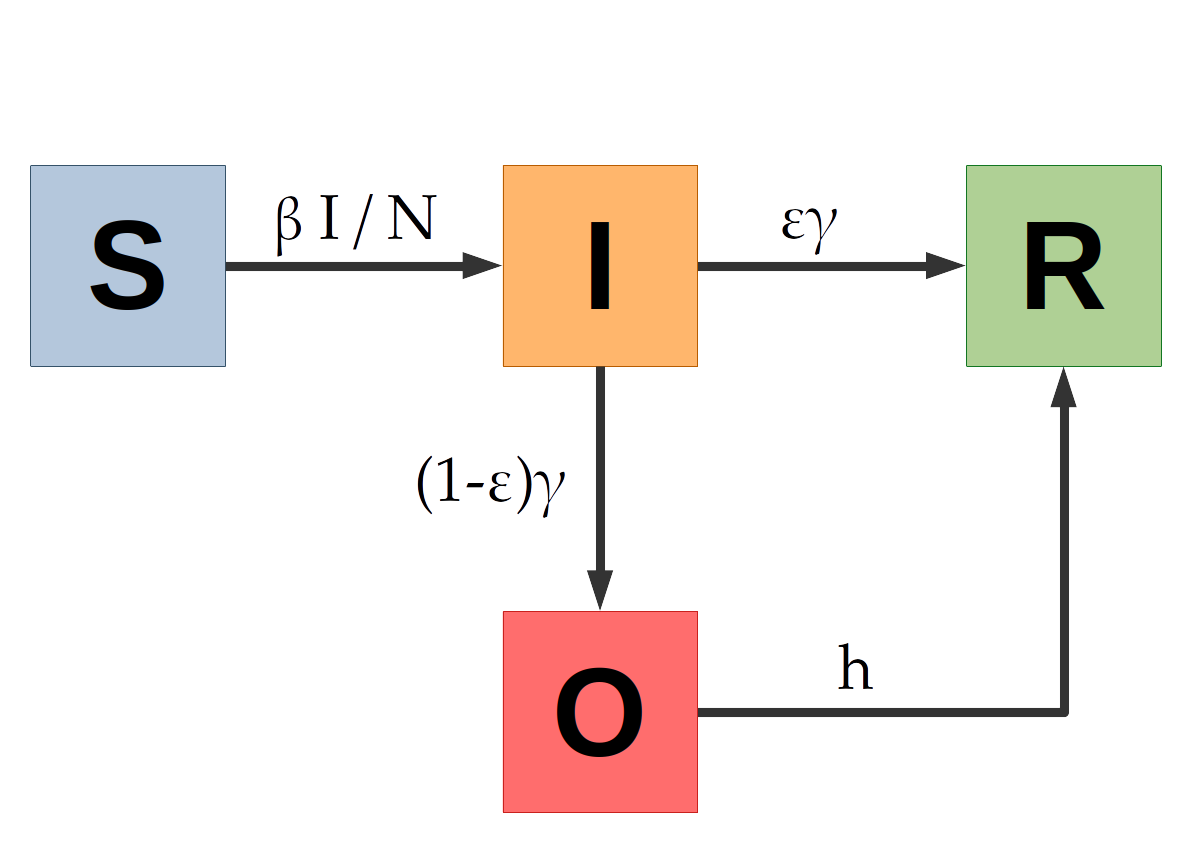
\includegraphics[width=0.7\columnwidth]{SIOR}
\par\end{centering}
\caption{Compartimental model}
\end{figure}


\section{Lockdown}

We notice a strong lockdown effect from mobility data
\begin{figure}[H]
\begin{centering}
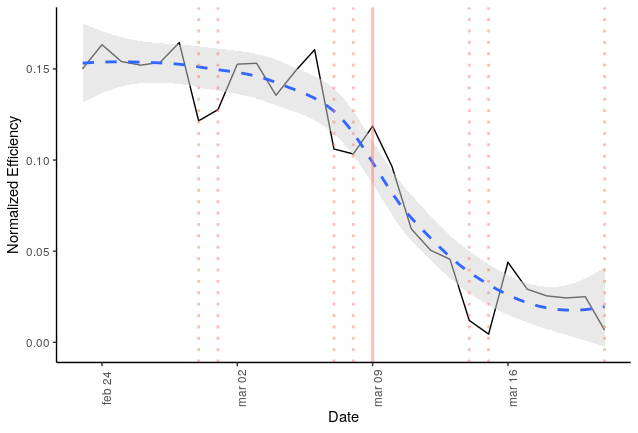
\includegraphics[width=0.7\columnwidth]{MobilityLockDown}
\par\end{centering}
\caption{Mobility change}
\end{figure}

To fit our model over Italian data, i.e., we confront $Y^{obs}$,
the reported cumulative number of Covid19 cases, with a fraction $\omega$
of the analogous quantity $Y^{mod}$ predicted by our model. We observe
a good stability of the fitted parameters (i.e. they change by few
percent by varying $\omega$ in a range $[10\%\ldots100\%]$).
\begin{figure}[H]
\begin{centering}
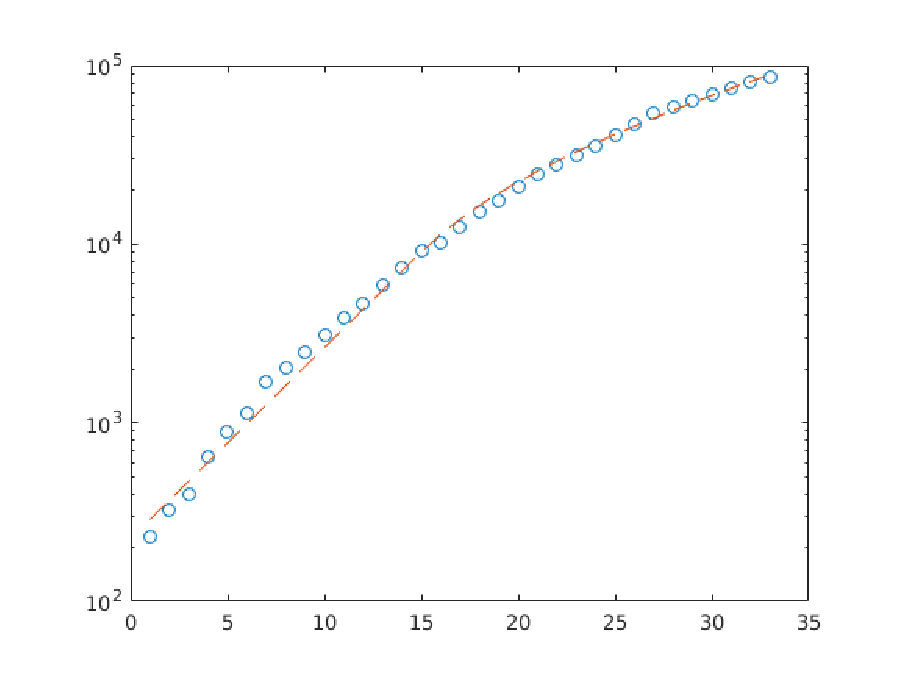
\includegraphics[width=0.7\columnwidth]{FitAttenuation}
\par\end{centering}
\caption{Comparison of the cumulative number of observed cases with our model.
Parameters indicate a reduction of $50\%$ in the number of contacts
after the lockdown}
\end{figure}
To take account of a possible reduction of the virality due to reduced
contacts, we consider two different values $\beta^{I},\beta^{II}$
before and after the lockdown. We find $\beta^{I}/\beta^{II}\sim50\%$;
such results indicate that , thanks to the reduction in mobility and
the new social distance behaviors, such reduction correspond to a
$\sim50\%$ post-lockdown decrease in contacts. The number does not
depend significantly on the fraction $\omega$ of serious cases we
are observing. 

\section{Scenarios}

The observed reproduction number in our model is $R_{0}\sim3.5$ and
is again stable against varying the fraction $\omega$ of cases. Notice
that in our model $\beta$ (and hence $R_{0}$) depends also on the
contact matrix $C$, i.e. on the structure of social interactions
among age classes; as an example, the different patterns of contacts
in Germany and in Italy could easily justify a growth of the epidemic
twice faster in the second country.

We first consider what happens by stopping the lockdown after the
peak of reported synthomatic people (i.e. $\omega O$) 
\begin{figure}[H]
\begin{centering}
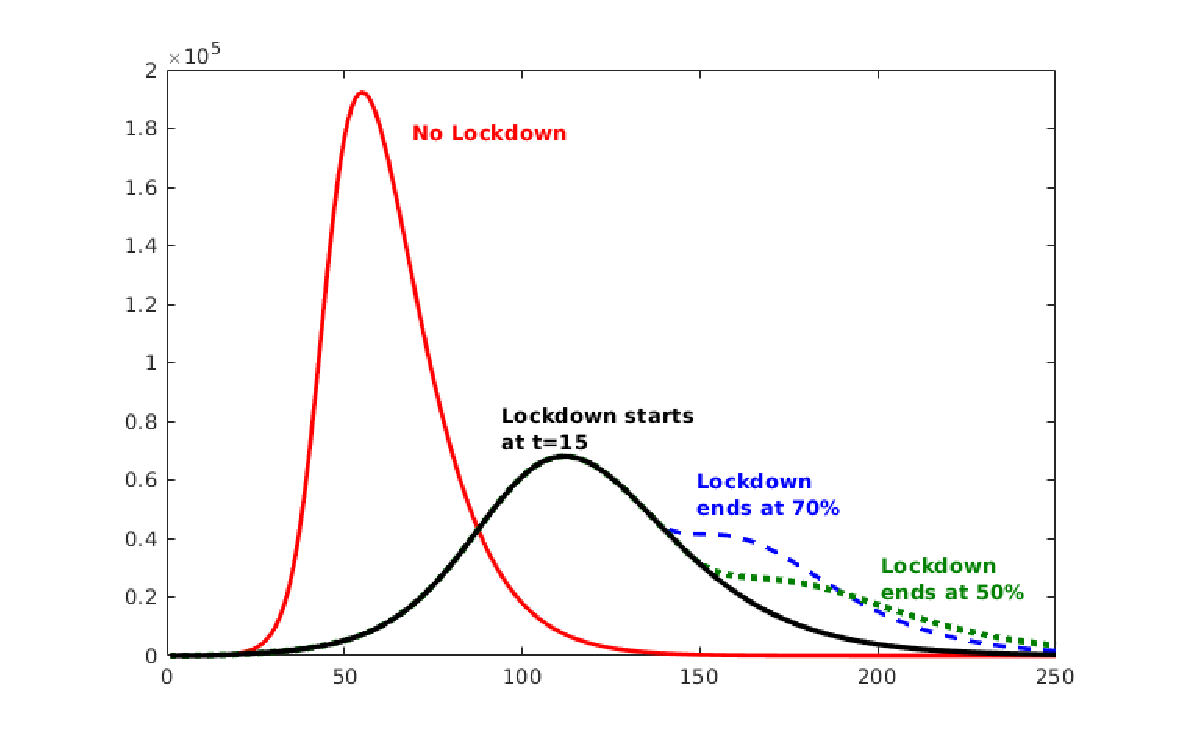
\includegraphics[width=0.7\columnwidth]{Scenario1}
\par\end{centering}
\caption{Comparison of the scenarios where the lockdown is relaxed after it
is reached the $70\%$ and the $50\%$ of the reported cases peak}
\end{figure}

We notice that, contrary to the scenarios were exiting the lockdown
would restart the epidemics and create a new peak, for our parameters
exiting the lockdown prolongs the reporting of cases without putting
under strain the national healthcare system (HERE WE ARE AVOIDING
SPEAKING OF THE MORTALITY .... THAT COULD BE THE FOCUS OF THE PAPER:
SCENARIOS FOR HEALH-CARE CAPACITY). This is due to the fact that,
in our model and with our estimated parameters (remember $R_{0}\sim3.5$),
the number of infected and recovered is much higher than what reported
to the national healthcare system. Hence, lockdown does not happen
in the early stages .

Notice that lockdown has two effects: lowering the peak -- very important
for avoiding the collapse pf the national healthcare system -- but
also moving the peak toward later times -- extremely obnoxious for
the economy of a country. 

\subsection{Early Lockdown}

Here we show that early lockdown reduce the height of the peak without
much moving it forward in time. However, ending the lockdown can make
epidemic start again

\subsection{Strong lockdown}

Here we show that increasing the strength of the lockdown (i.e. reducing
the social contacts) is much less effective than acting in early times;
moreover, if moves the peak forward in time. It can be reasonable
only for low productive part of the population

\subsection{Effects on regions}

Starting from the fact that different regions have different delays
in the start of the epidemics (taking Lombardia as the earliest),
we could analyze possible scenarios according to the delay (i.e. can
the end of the lockdown restart an epidemic in some regions?)

\section{Class Ages}

The model, to take account for age classes, incorporates also contact
patterns through a sociological matrix $C$ that rescales the infectivity
$\beta$; moreover, it also considers the different age incidence
of ``observable'' cases through a matrix $\varXi$ that built up
on ISS data.

\section{Some thoughts}

Social matrices indicates that
\begin{itemize}
\item Young people ($0-19$) are the most interconnected, with higher contacts
rates. They are the ones that ``dominate'' $R_{0}$. Hence, most
policies will be late if they don't act first with youngs. On the
other hand, if the infection is very quick and mostly asymptomatic,
it is difficult to detect an epidemic before it has already spread
too much
\item Elderly people ($60+$) are the second most interconnected class.
Since for Covid19 the incidence is also higher in their class, that's
were it makes sense to enforce a stronger and longer lockdown
\end{itemize}
Thnks
\end{document}
